%**************************************************************************************
% License:
% CC BY-NC-SA 4.0 (http://creativecommons.org/licenses/by-nc-sa/4.0/)
%**************************************************************************************

\documentclass[notes]{beamer}

\mode<presentation> {

\usetheme{Madrid}

% Burnt orange
\definecolor{burntorange}{rgb}{0.8, 0.33, 0.0}
\colorlet{beamer@blendedblue}{burntorange}
% Pale yellow
\definecolor{paleyellow}{rgb}{1.0, 1.0, 0.953}
\setbeamercolor{background canvas}{bg=paleyellow}
% Secondary and tertiary palett
\setbeamercolor*{palette secondary}{use=structure,fg=white,bg=burntorange!80!black}
\setbeamercolor*{palette tertiary}{use=structure,fg=white,bg=burntorange!60!black}

% To remove the footer line in all slides uncomment this line
%\setbeamertemplate{footline}
% To replace the footer line in all slides with a simple slide count uncomment this line
%\setbeamertemplate{footline}[page number]

% To remove the navigation symbols from the bottom of all slides uncomment this line
%\setbeamertemplate{navigation symbols}{}
}

\usepackage{amsmath}
\usepackage{bm}
\usepackage{breqn}
\usepackage{fontawesome}
\usepackage{graphicx} % for figures
\usepackage{subcaption} % for subplots 
\usepackage[labelsep=space,tableposition=top]{caption}
\renewcommand{\figurename}{Fig.} 
\usepackage{cleveref}
\usepackage{caption,subcaption}% http://ctan.org/pkg/{caption,subcaption}
\usepackage{booktabs} % Allows the use of \toprule, \midrule and \bottomrule in tables
\usepackage{multirow}
\usepackage{xcolor}
\usepackage{empheq}
\usepackage[most]{tcolorbox}
\usepackage{listings}% http://ctan.org/pkg/listings
\lstset{basicstyle=\ttfamily,breaklines=true}
\usepackage{siunitx}
\usepackage{verbatim}

% To print 2 slides on a page
%\usepackage{handoutWithNotes}
%\pgfpagesuselayout{2 on 1}[border shrink=2mm]
%----------------------------------------------------------------------------------------
%	TITLE PAGE
%----------------------------------------------------------------------------------------
% The short title appears at the bottom of every slide, the full title is only on the title page
\title[CE 311K: Control flow]{CE 311K: Control flow} 
\author{Krishna Kumar} % name
\institute[UT Austin] % institution 
{
University of Texas at Austin \\
\medskip
\href{mailto:krishnak@utexas.edu}{krishnak@utexas.edu} % email address
}
\date{\today} % Date, can be changed to a custom date

\begin{document}

\begin{frame}
\titlepage % title page as the first slide
\end{frame}

\newif\ifshowtoc
\showtoctrue% toggles to show the toc

\AtBeginSection{%
	\ifshowtoc
	\begin{frame}
		\tableofcontents[currentsection, subsectionstyle=show/show/hide]
	\end{frame}
	\fi
}

%----------------------------------------------------------------------------------------
% slides
%----------------------------------------------------------------------------------------
%------------------------------------------------

\section{Numerical solution}
%------------------------------------------------
\subsection{Numerical solution of a sliding block}
\begin{frame}
	\frametitle{What is the optimal angle to pull the statue?}
	\begin{figure}[ht]
		\centering
		\includegraphics[width=\textwidth]{figs/egypt-pyramid.jpg}
		\caption*{A wall painting from the tomb of Djehutihotep (credit: martinhumanities.com)}
	\end{figure}
\end{frame}

%------------------------------------------------
\begin{frame}
	\frametitle{Numerical solution of a sliding block: Approximation}
	\begin{figure}[ht]
		\centering
		\includegraphics[width=0.85\textwidth]{figs/sliding-block.png}
		\caption*{What is the optimal angle to pull the block applying the least amount of force?}
	\end{figure}
\end{frame}


%------------------------------------------------
\begin{frame}
	\frametitle{Numerical solution of a sliding block: Forces}
	\mode<beamer>{		
		\begin{figure}[ht]
			\centering
			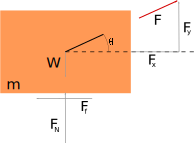
\includegraphics[width=0.85\textwidth]{figs/block-forces.png}
		\end{figure}
	}
	\mode<handout>{
		\begin{figure}[ht]
			\centering
			\includegraphics[width=0.85\textwidth]{figs/block-noforces.png}
		\end{figure}
	}
\end{frame}


%------------------------------------------------
\begin{frame}
	\frametitle{Numerical solution of a sliding block: Forces}
	\begin{minipage}[t]{0.7\linewidth}
		\mode<beamer>{		
			\begin{align*}
			& F_x = F \cos \theta \quad \& \quad F_y = F \sin \theta\\
			& F_f = \mu \cdot F_N = \mu \cdot W - \mu F_y = \mu m g - \mu F \sin \theta \\
			& \text{Vertical forces} \sum F_{vert} \uparrow: F_y + F_N - W = 0 \\
			& F_N = \mu m g - F \sin \theta \\
			& \text{Horizontal forces} \sum F_{hor} \rightarrow: F_x + F_f = 0 \\ 
			& F \cos \theta - \mu m g + \mu F \sin \theta = 0 \\
			\end{align*}
		}
		\mode<handout>{
			\vspace{4cm}
		}
	\end{minipage}%
	\hfill%
	\begin{minipage}[t]{0.29\linewidth}
		\begin{figure}[ht]
			\centering
			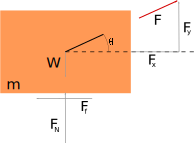
\includegraphics[width=\textwidth]{figs/block-forces.png}
		\end{figure}
	\end{minipage}%
	
	\begin{empheq}[box=\tcbhighmath]{equation*}
	F = \frac{\mu \cdot m g}{(\cos \theta + \mu \sin \theta)}
	\end{empheq}
\end{frame}

%------------------------------------------------
\begin{frame}
	\frametitle{Numerical solution of a sliding block: Compute force}
	\begin{itemize}
		\item Given $W = 25 kN (\SI{2500}{kg})$, $\theta = 45^o$ and $\mu = 0.75$ ($35^o$):
		\mode<beamer>{	
			\begin{equation*}
			F = \frac{0.75 \times 25 }{\cos(45) + 0.75 \sin(45)} = \SI{15.15}{kN}.
			\end{equation*}
		}
		\mode<handout>{
			\vspace{1.5cm}
		}
		\item Given $F = 17.5 kN (\SI{1750}{kg})$ and $\mu = 0.75$, what's $\theta$?
		\begin{figure}[ht]
			\centering
			\includegraphics[width=0.6\textwidth]{figs/sliding-block-mu0p75.png}
		\end{figure}
	\end{itemize}
\end{frame}


%------------------------------------------------
\begin{frame}
	\frametitle{Numerical solution of a sliding block: Compute force}
	\begin{itemize}
		\item Given $F = 17.5 kN (\SI{1750}{kg})$ and $\mu = 0.75$, what's $\theta$?
		\mode<beamer>{	
			\begin{align*}
			Try~\theta = 60^o:~ & F = \frac{0.75 \times 25 }{\cos(60) + 0.75 \sin(60)} = \SI{16.31}{kN}.\\
			Try~\theta = 70^o:~ & F = \frac{0.75 \times 25 }{\cos(70) + 0.75 \sin(70)} = \SI{17.91}{kN}.\\
			Try~\theta = 65^o:~ & F = \frac{0.75 \times 25 }{\cos(65) + 0.75 \sin(65)} = \SI{17.00}{kN}.\\
			Try~\theta = 67,5^o:~ & F = \frac{0.75 \times 25 }{\cos(67.5) + 0.75 \sin(67.5)} = \SI{17.43}{kN}.
			\end{align*}
			This is \textbf{bisection method!}
		}
		\mode<handout>{
			\vspace{4cm}
		}
	\end{itemize}
\end{frame}


%------------------------------------------------
\begin{frame}
	\frametitle{\faCommentsO ~What are the characteristics of a numerical solution?}
	\mode<beamer>{
		\begin{itemize}
			\item A numerical recipe is \textit{a sequence of simple steps}
			\item \textit{Flow of control} as each step is executed.
			\item Yields an \textit{approximate} numerical answer (a finite number) for the problem 
			\item These solutions can be very accurate
			\item Most answers are determined in an iterative approach (numerical method: mathematical / computer-aided technique) until a desired minimum/acceptable accuracy is obtained
			\item Typically, a finite set of iterations (steps) are used in the numerical method to obtain a solution. A means of determining \textit{when to stop}.
		\end{itemize}
	}
	\mode<handout>{
		\vspace{5cm}
	}
\end{frame}

%------------------------------------------------
\begin{frame}
	\frametitle{Numerical solution of a sliding block: Friction angles}	
	\begin{figure}[ht]
		\centering
		\includegraphics[width=0.85\textwidth]{figs/sliding-block-force-frictions.png}
	\end{figure}
\end{frame}

\end{document}